\documentclass[11pt]{article}

\usepackage[margin=1in]{geometry}
\usepackage{amsmath,amssymb}
\usepackage{graphicx}
\usepackage{float}
\usepackage{booktabs}
\usepackage{hyperref}
\usepackage{natbib}
\usepackage{authblk}
\usepackage[T1]{fontenc}
\usepackage{times}

\hypersetup{
  colorlinks=true,
  linkcolor=blue,
  citecolor=blue,
  urlcolor=blue
}

\title{Language Cadence: A Null Result}
\author{Navid Nabijou}
\date{September 24, 2026}

\begin{document}

\maketitle

\begin{abstract}
Positional encodings in transformer language models are usually language-agnostic: the original geometric encoding of \citet{vaswani2017attention} uses a fixed spread of frequencies regardless of what is being modeled. This work asks a narrower question: if a strictly \emph{periodic} positional encoding is used instead, does tuning its period per language improve next-token pretraining loss in an otherwise-fixed, from-scratch GPT? The idea has some loose motivation from linguistics --- languages are sometimes claimed to differ in rhythmic timing --- but the experiment is evaluated purely on pretraining loss, independent of whether that linguistic distinction holds up. We sweep the period across 14 values and five languages (English, French, German, Italian, Spanish; 70 runs total) and find no benefit from per-language tuning: for every language, test loss decreases monotonically as the period grows, all the way to the model's context length. This is a boundary effect rather than a genuine positional optimum --- a long period simply gives the model more usable context within a fixed window, rather than encoding any exploitable periodic structure. Supporting this reading, a geometric property of the encoding explicitly designed to penalize very long periods turns out to be \emph{positively} correlated with test loss across the sweep (Pearson $r = +0.930$), the opposite of what that design predicts. We report this as a null result and identify the character-level tokenizer used here as a likely reason the underlying idea was not given a fair test.
\end{abstract}

\section{Introduction}

Standard positional encodings for transformers do not repeat: the geometric frequency spread introduced by \citet{vaswani2017attention} spans a wide range of wavelengths and never returns exactly to a previous value within any practical sequence length. This project asks what happens if that property is dropped --- if the positional encoding is instead made strictly periodic, with a period $P$ chosen per language --- and whether tuning $P$ can improve next-token pretraining loss for a small, from-scratch GPT.

The motivation is partly architectural: a language-specific positional encoding would be a cheap lever if it worked, requiring no change to the rest of the model. It also has loose support from linguistics. Phonetics has long debated whether languages fall into rhythmic classes --- ``stress-timed'' languages such as English and German versus ``syllable-timed'' languages such as French, Spanish, and Italian --- with a regular interval, or isochrony, underlying each class. The empirical case for measurable acoustic isochrony is weak: studies measuring inter-stress or inter-syllable intervals have repeatedly failed to separate languages cleanly along these lines. We treat this debate only as motivation for trying a per-language period sweep, not as something this experiment tests or assumes; the result below stands or falls on pretraining loss alone.

Concretely, a GPT architecture is fixed and only the positional encoding $\mathbf{\Pi}$ is varied. $\mathbf{\Pi}$ is combined with the token-embedding matrix $\mathbf{X}$ (both $D \times N$, where $D$ is the embedding dimension and $N$ is the context length) to inject position information into the model. The question is whether some period $P^{*}$ consistently minimizes next-token test loss for a given language, and whether $P^{*}$ differs meaningfully across languages.

Two effects could produce a misleading answer to this question, and the experiment below is designed with both in mind. First, a positional encoding with period $P$ close to the context length $N$ stops repeating within any single training window --- at that point, increasing $P$ further is effectively equivalent to giving the model a longer usable context, which improves loss for reasons that have nothing to do with periodicity. We call this the \emph{boundary effect}: any sweep that includes $P$ values approaching $N$ risks measuring this instead of a genuine positional optimum, and the sweep below deliberately includes $P = N$ as a direct check for it. Second, if a language's text is tokenized in a way that only loosely tracks its actual structure --- for instance, one character per token, regardless of orthographic depth --- then any period found to work well could be an artifact of tokenization efficiency rather than a real, exploitable effect; we return to this concern in Section~\ref{sec:limitations}.

\section{Method}

\subsection{Positional Encoding}
\label{sec:pe}

Each position $n \in \{0, \dots, N-1\}$ is encoded by one column of $\mathbf{\Pi}$, a $D$-dimensional vector built from $H = D/2$ row-pairs, each pair holding a $(\sin, \cos)$ value at some frequency. A sine/cosine pair traces out a point on a unit circle as $n$ advances, so relative positions can in principle be recovered from a pair via a simple rotation --- the same property that motivates the sinusoidal pairing in \citet{vaswani2017attention}'s original encoding. What differs here is that the frequencies are chosen so that the whole matrix has an exact period $P$, i.e.\ $\mathbf{\Pi}(n) = \mathbf{\Pi}(n+P)$ for every $n$: a sinusoid sampled only at integers is exactly periodic with period $P$ whenever its frequency is an integer multiple of $2\pi/P$, so row-pair $j$ is assigned an integer \emph{harmonic number} and oscillates at $\sin(2\pi \cdot \text{harmonic} \cdot n / P)$ and $\cos(2\pi \cdot \text{harmonic} \cdot n / P)$.

The one complication is that not every integer harmonic gives a genuinely new pattern. For integer $n$,
\[
  \sin\!\left(\frac{2\pi (P-k) n}{P}\right) = \sin\!\left(2\pi n - \frac{2\pi k n}{P}\right) = -\sin\!\left(\frac{2\pi k n}{P}\right),
\]
using $\sin(2\pi n - x) = -\sin(x)$, which holds because $n$ is an integer. So harmonic $P-k$ traces out exactly the same shape as harmonic $k$, up to an overall sign, and the two carry essentially the same positional information. If row-pairs were simply assigned harmonics $j = 1, 2, 3, \dots$ in order, every row-pair with $j > P/2$ would duplicate (up to sign) an earlier one, wasting embedding capacity on redundant rows once $j$ ran past that point. To avoid this, each row-pair $j$ is instead assigned the \emph{folded} harmonic
\[
  k_j = \min(j \bmod P,\; P - (j \bmod P)),
\]
which maps $j$ onto the fundamental range $\{0, 1, \dots, \lfloor P/2 \rfloor\}$ and only starts reusing a harmonic once every value in that range has already appeared. With this assignment,
\[
  \Pi[2j-2, n] = \sin\!\left(\frac{2\pi k_j n}{P}\right), \qquad
  \Pi[2j-1, n] = \cos\!\left(\frac{2\pi k_j n}{P}\right).
\]

\paragraph{A worked example.} To make this concrete, the block below shows $\mathbf{\Pi}$ for $P = 8$ --- one of the values used in the sweep (Section~2.4) --- restricted to its first six rows (row-pairs $j = 1, 2, 3$, with folded harmonics $k_1 = 1$, $k_2 = 2$, $k_3 = 3$; no folding has occurred yet at this $j$) and first six columns ($n = 0, \dots, 5$):
\[
\begin{pmatrix}
\sin 0 & \sin\tfrac{\pi}{4} & \sin\tfrac{\pi}{2} & \sin\tfrac{3\pi}{4} & \sin\pi & \sin\tfrac{5\pi}{4} \\
\cos 0 & \cos\tfrac{\pi}{4} & \cos\tfrac{\pi}{2} & \cos\tfrac{3\pi}{4} & \cos\pi & \cos\tfrac{5\pi}{4} \\
\sin 0 & \sin\tfrac{\pi}{2} & \sin\pi & \sin\tfrac{3\pi}{2} & \sin 2\pi & \sin\tfrac{5\pi}{2} \\
\cos 0 & \cos\tfrac{\pi}{2} & \cos\pi & \cos\tfrac{3\pi}{2} & \cos 2\pi & \cos\tfrac{5\pi}{2} \\
\sin 0 & \sin\tfrac{3\pi}{4} & \sin\tfrac{3\pi}{2} & \sin\tfrac{9\pi}{4} & \sin 3\pi & \sin\tfrac{15\pi}{4} \\
\cos 0 & \cos\tfrac{3\pi}{4} & \cos\tfrac{3\pi}{2} & \cos\tfrac{9\pi}{4} & \cos 3\pi & \cos\tfrac{15\pi}{4}
\end{pmatrix}
\]
Rows 0--1 are $(\sin, \cos)$ at $k_1 = 1$; rows 2--3 at $k_2 = 2$; rows 4--5 at $k_3 = 3$. Reading down a column gives the position-$n$ encoding contributed by each harmonic; reading across a row shows how each sinusoid's argument grows with $n$. Leaving the entries unevaluated makes the pattern easy to read off directly: row-pair 1's argument is $\tfrac{\pi n}{4}$; row-pair 2's is $\tfrac{\pi n}{2}$, twice as large at every $n$, so it already completes a full $2\pi$ turn by $n = 4$ (row-pair 1 has only reached $\pi$, half a turn, by then); row-pair 3's argument is $\tfrac{3\pi n}{4}$, three times row-pair 1's, and reaches $\tfrac{3\pi}{2}$ --- three-quarters of a turn, where $\sin$ is at its most negative --- already by $n = 2$. Higher-$k_j$ row-pairs simply advance through their cycle faster as $n$ increases.

\paragraph{Distinguishability.} That last observation is the basis for a purely geometric property of $\mathbf{\Pi}$, measurable without training anything: how much the encoding changes between adjacent positions. Define
\[
  \mathrm{dist}(P) = \frac{1}{P} \sum_{n=0}^{P-1} \big\lVert \mathbf{\Pi}(:, (n+1) \bmod P) - \mathbf{\Pi}(:, n) \big\rVert_2,
\]
the mean $L_2$ distance between neighboring position-columns, averaged over one full period (including the wrap-around pair, since $\mathbf{\Pi}$ is exactly periodic). A small $\mathrm{dist}(P)$ means adjacent positions look nearly identical to the encoding, and a model reading it would find neighboring tokens' positions hard to tell apart; a large $\mathrm{dist}(P)$ means adjacent positions are easy to distinguish.

$\mathrm{dist}(P)$ is not monotonic in $P$, and the reason is the trade-off implicit in the construction above. When $P$ is small, only $\lfloor P/2 \rfloor + 1$ distinct folded harmonics exist, so with $H = 32$ fixed, most row-pairs are forced to repeat an already-used harmonic (up to sign) --- including, for the smallest $P$, several row-pairs stuck at $k_j = 0$, which is constant in $n$ and contributes nothing to distinguishing positions at all. Embedding capacity is spent on redundant or uninformative rows, so distinguishability suffers even though the few genuinely distinct harmonics present oscillate quickly. When $P$ is large, by contrast, $j$ never exceeds $P/2$ for any of the $H = 32$ row-pairs actually used, so folding never triggers and every row-pair gets a distinct harmonic $k_j = j$ --- but each harmonic's angular step from one position to the next is $2\pi k_j / P$, which shrinks as $P$ grows for every fixed $k_j$. With no harmonic higher than $H$ available, even the fastest row-pair advances by only $2\pi H / P$ radians per step, so for large enough $P$ every row-pair changes almost imperceptibly from one position to the next, and $\mathrm{dist}(P)$ falls again. Between these two regimes --- too few distinct harmonics, and too-slow harmonics --- there is an interior value of $P$ where distinguishability is maximized; for $H = 32$ ($D = 64$), this was confirmed numerically to occur at $P \approx 45$, refined during implementation to scale as roughly $1.4H$ across a range of $H$ values, rather than the naive $P \approx 2H$ that the aliasing argument alone would suggest.

\paragraph{Why build this trade-off in deliberately.} The point of constructing $\mathbf{\Pi}$ this way, rather than using an arbitrary periodic function, is that it yields a clean, purely geometric prediction to test trained behavior against. If a model's ability to use positional information is genuinely limited by how distinguishable nearby positions are in the encoding, next-token test loss should be minimized somewhere near the period that maximizes $\mathrm{dist}(P)$, and should worsen as $P$ moves away from that point in either direction --- independent of any language-specific effect. This makes the geometric optimum a natural, pre-computable reference point for interpreting the sweep: a result that tracks it would be consistent with distinguishability driving performance, while a result that does not would point to some other mechanism. Section~\ref{sec:experiments} reports which of these actually happens.

How $\mathbf{\Pi}$ combines with the token embedding $\mathbf{X}$ was resolved by a small calibration experiment (7 short English-only runs at $P = 45$, comparing additive injection $\mathbf{X} + a\mathbf{\Pi}$ across amplitudes $a \in \{0, 0.1, 0.25, 0.5, 1, 2, 4\}$ against concatenation, $\mathrm{Linear}(\mathrm{concat}(\mathbf{X}, \mathbf{\Pi}))$). Additive injection at amplitude $0.1$ reached the lowest loss in this small comparison ($2.243$), only narrowly ahead of concatenation ($2.264$); amplitude also turned out to have a narrow, saturating sweet spot, since every transformer block here opens with LayerNorm and $\mathrm{LayerNorm}(cv) = \mathrm{LayerNorm}(v)$ for any positive scalar $c$ --- amplitudes of $2$ and $4$ produced identical eval-loss curves to three decimal places. Concatenation sidesteps this fragility entirely, at the cost of one extra learned projection layer, and was used for the full sweep reported below.

\subsection{Tokenizer and Preprocessing}

Text is tokenized at the character level, restricted to English, French, German, Italian, and Spanish; inputs are NFC-normalized and lowercased, with a single 64-symbol vocabulary shared across all five languages (the 26 unaccented Latin letters, 15 accented or language-specific letters spanning the five languages, 10 digits, 11 punctuation marks, whitespace, and \texttt{<UNK>}) and rare characters folded into \texttt{<UNK>}. This choice is revisited critically in Section~\ref{sec:limitations}.

\subsection{Dataset}

Training data is drawn from Europarl (European Parliament Proceedings Parallel Corpus), with a document-level train/test split (10\% of documents held out per language) to avoid leakage; documents are fixed 500-sentence chunks, since the Europarl v7 release has no native chapter markup. Windows of 384 non-overlapping characters are used throughout, giving $\sim$17.6--18.0M training characters and $\sim$1.8--2.0M test characters per language. Because Europarl is a translated, sentence-aligned corpus, it carries a known ``translationese'' risk --- source-language structural traces bleeding into the target --- that could damp any real per-language signal; a planned robustness check against an independently-sourced monolingual corpus (e.g.\ native Wikipedia) was not run for this write-up.

\subsection{Architecture and Sweep}

The model is a small GPT: embedding dimension $D = 64$, $H = 32$ positional-encoding row-pairs (not to be confused with the model's 4 attention heads, a separate quantity), 4 layers, 4 attention heads, concatenation injection, and context length $N = 384$, held fixed across the whole sweep. The period is swept over
\[
  P \in \{3, 4, 6, 8, 16, 24, 32, 45, 64, 96, 128, 192, 256, 384\},
\]
spanning below and above the geometric peak $P = 45$, and including $P = 384 = N$ exactly --- the direct test for the boundary effect described in Section~1, since a period equal to the context window makes periodicity structurally unobservable within one window. With 5 languages $\times$ 14 $P$ values $\times$ 1 seed, this gives 70 runs, each trained for $\sim$3000 steps at batch size 16 ($\approx$ 18.4M characters, close to one full epoch over a language's training set). Final loss is reported on the full held-out test set once at the end of training, not on the smaller subset used for periodic eval-time tracking.

\section{Experiments}
\label{sec:experiments}

\textbf{No language shows a genuine positional optimum: loss simply improves with $P$, all the way to the context length.} For all five languages, test loss decreases monotonically across the entire tested range and reaches its minimum at $P = 384$, the largest value tested and exactly equal to the context length $N$. None of the five languages shows an interior minimum.

\begin{figure}[H]
  \centering
  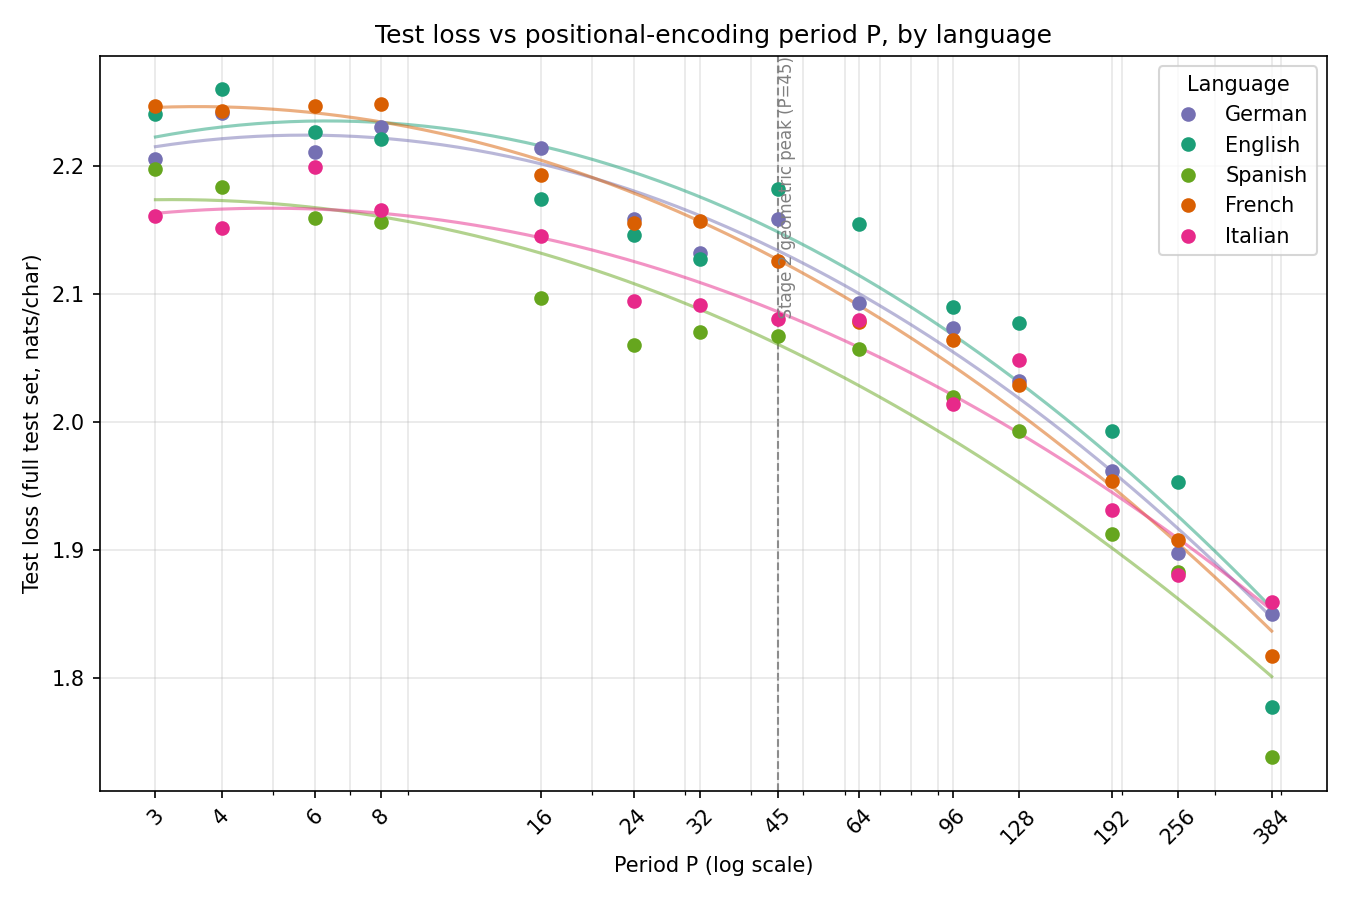
\includegraphics[width=\textwidth]{../figures/sweep_test_loss_vs_P.png}
  \caption{Test loss vs.\ $P$ (log-$x$), one line per language. All five decrease monotonically to $P = 384 = N$.}
  \label{fig:sweep}
\end{figure}

\begin{table}[H]
  \centering
  \caption{Test loss at $P = 384$ (the lowest observed, at the context-length boundary) vs.\ $P = 45$ (the period that maximizes the encoding's own geometric distinguishability), by language.}
  \label{tab:results}
  \begin{tabular}{lcc}
    \toprule
    Language & Loss at $P = 384$ & Loss at $P = 45$ \\
    \midrule
    Spanish  & 1.738 & 2.067 \\
    English  & 1.777 & 2.182 \\
    French   & 1.817 & 2.126 \\
    German   & 1.850 & 2.159 \\
    Italian  & 1.859 & 2.080 \\
    \bottomrule
  \end{tabular}
\end{table}

Loss at $P = 45$ --- the period favored by the encoding's own geometric design --- is worse than at every larger $P$ tested, for every language. This is the pattern expected from a boundary effect: performance keeps improving as $P$ approaches $N$, rather than peaking at some interior value and declining again.

A few languages show small local dips at interior $P$ values that are not the overall minimum --- German at $P = 6$ and $P = 32$, English at $P = 32$, Spanish at $P = 24$, French at $P = 4$ and $P = 24$, Italian at $P = 4$ and $P = 96$. These do not cluster near $P = 45$ or any other single value across languages, and with only one training run per $(P, \text{language})$ pair, this is consistent with ordinary run-to-run noise. They are reported here for completeness, not as evidence of a real per-language effect.

\textbf{The encoding's own geometric design predicts the opposite of what is observed.} $\mathbf{\Pi}$ was constructed so that an overly long period makes neighboring positions harder to distinguish from one another --- this ``distinguishability'' metric peaks at $P = 45$ (score $8.895$ for $D = 64$) and falls roughly $5\times$ by $P = 384$ (score $1.738$), the worst point on the grid. If that geometric property mattered for trained performance, distinguishability and test loss should move in \emph{opposite} directions as $P$ varies. They do not: computed over the 14-point $P$ grid, the Pearson correlation between distinguishability and mean test loss is $\boldsymbol{r = +0.930}$ --- strongly positive, the opposite sign from what the ``distinguishability drives performance'' hypothesis predicts. $P = 45$ (distinguishability $8.895$) has mean test loss $2.123$; $P = 384$ (distinguishability $1.738$, the worst on the grid) has mean test loss $1.808$, the best on the grid.

\begin{figure}[H]
  \centering
  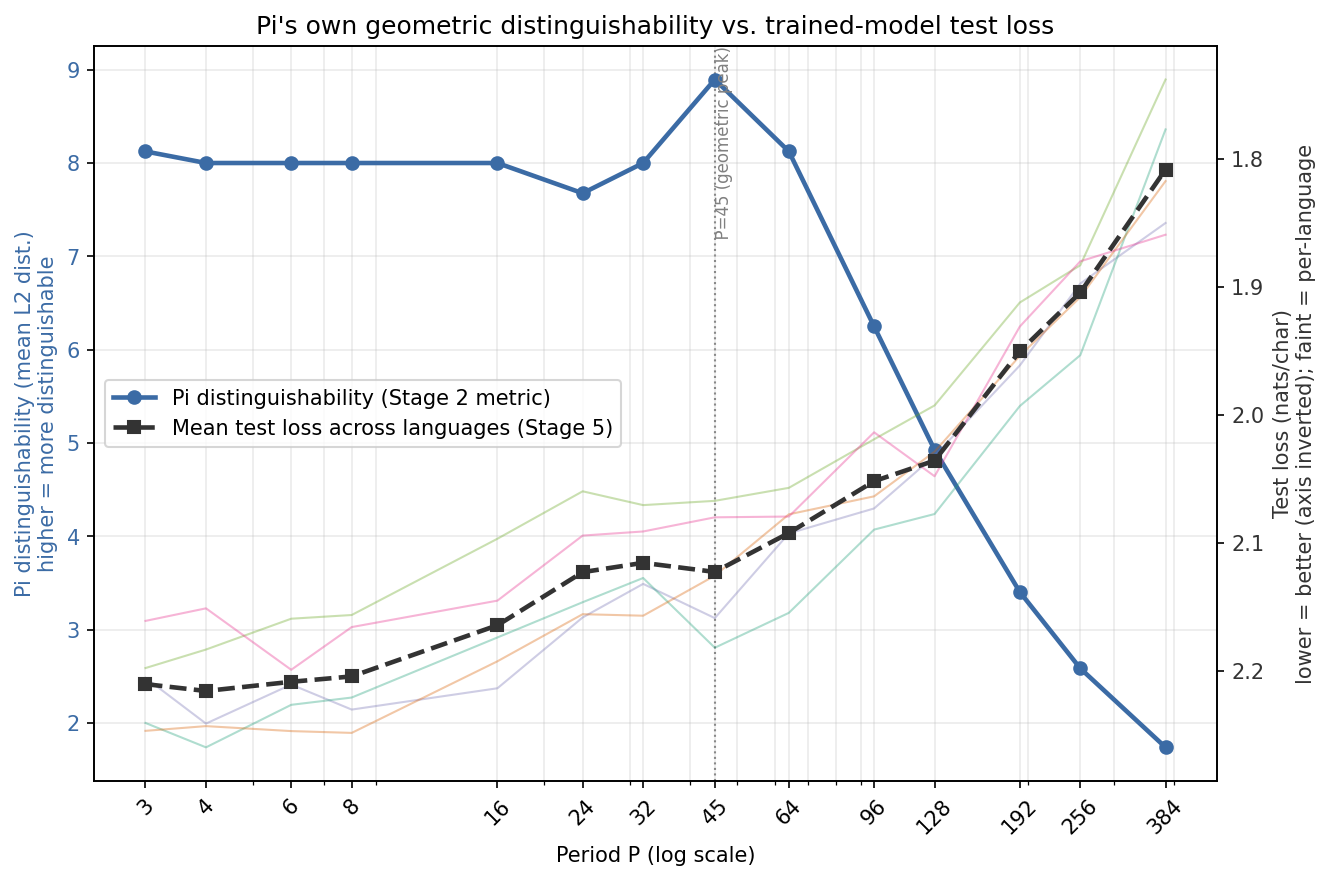
\includegraphics[width=\textwidth]{../figures/distinguishability_vs_loss.png}
  \caption{$\mathbf{\Pi}$'s geometric distinguishability and mean test loss, plotted over the same $P$ grid. Pearson $r = +0.930$.}
  \label{fig:distinguishability}
\end{figure}

In other words, the specific mechanism the encoding was engineered around --- protecting against overly long periods via an adjacent-position distinguishability penalty --- had no apparent benefit in the trained models, and was maximally active exactly where they performed best.

\textbf{The result is best explained by the boundary effect, not a failed positional signal.} A larger $P$ means $\mathbf{\Pi}$ repeats less within a single 384-token window, giving the model access to more distinguishable positional information regardless of whether that period bears any relationship to the language being modeled. That is exactly the pattern observed for all five languages, with no exceptions, and $P = 384 = N$ --- included specifically to test for this --- wins by a wide margin every time. At the scale tested here (fixed $N = 384$, a single training seed, roughly one epoch), the experiment cannot distinguish ``a genuinely better positional encoding at this specific period'' from ``more usable context, up to the boundary.'' A cleaner test would keep the swept $P$ range well below $N$ --- for example, using a much larger context length so that even the largest tested $P$ is a small fraction of it --- leaving room for a genuine interior optimum to appear if one exists.

\section{Limitations}
\label{sec:limitations}

\textbf{The character-level tokenizer likely understated the idea's chances.} Character-level tokenization avoids one obvious pitfall --- results depending on how efficiently a subword tokenizer happens to compress a given language --- but a character has no principled relationship to the structure of natural language. Digraphs and orthographic depth (German ``sch,'' English ``th,'' French nasal-vowel spellings) mean that a fixed number of characters corresponds to a different amount of actual linguistic structure in each language, and more importantly, a character is not a stable proxy for a syllable, mora, or foot --- the units any exploitable per-language positional signal would plausibly need to operate over. This is not merely a hunch: independent work on written-text rhythm metrics (Section~\ref{sec:related}) finds that apparent ``rhythm'' correlates with syllable/word-structure statistics rather than timing per se, which suggests the unit of tokenization is not a minor detail here but close to the whole question. Measuring periodicity over characters was, in that sense, close to measuring the wrong thing, independent of the boundary effect discussed above. A syllable- or morpheme-level tokenizer would let a candidate period $P$ be interpreted in linguistically meaningful units, which character counts cannot support across languages with different orthographic depth.

\textbf{The translationese question remains open.} Rerunning the best-performing $P$ values on an independently-sourced monolingual corpus per language, to check whether Europarl's translated text was damping a real signal, was never carried out, since the sweep did not produce per-language optima worth checking in the first place. This remains untested, not ruled out.

\section{Related Work}
\label{sec:related}

No prior work was found running this exact experiment --- sweeping a fixed periodic positional-encoding period in a from-scratch character-level GPT and reading off a per-language optimal $P$ from next-token test loss --- so this appears to be a novel combination, not a replication of an established method. The closest precedents:

\begin{enumerate}
  \item \citet{ghosh2024morphology} ablated positional encoding in pretrained monolingual BERT models across 22--23 languages on five downstream tasks, and found PE importance diminishes with increasing morphological complexity, with languages clustering by morphological typology. This is the closest ML precedent for ``PE matters differently by language,'' but it uses binary nullification on fine-tuned downstream tasks with a standard (non-periodic) PE, not a period sweep on a from-scratch next-token LM.
  \item A formal-language-theoretic result: a period-2 positional encoding solves the formal language $(aa)^{*}$ but fails on $(aaaa)^{*}$, i.e.\ a periodic PE's usefulness is tied to matching the data's actual periodic structure. This gives theoretical grounding for period-matching, but for synthetic formal languages, not natural language.
  \item \citet{stojanovic2013crosslinguistic} computed structural-complexity measures from written-text transcriptions across 21 languages and found several rhythm metrics strongly correlate with phonotactic complexity --- suggesting apparent ``rhythm'' may reflect syllable/word-structure statistics rather than timing per se. This is direct supporting evidence for the tokenization concern raised in Section~\ref{sec:limitations}.
  \item \citet{pellegrino2011crosslanguage}, using near-identical languages to this project's set (French, English, German, Spanish, Italian), found a trade-off between per-syllable information density and speech rate that roughly equalizes bits-per-second across languages. This is real, replicated evidence of a cross-linguistic timing-adjacent regularity, though framed as a rate/density trade-off rather than periodicity --- a useful contrast even though the stress-timed/syllable-timed dichotomy itself doesn't hold up well empirically.
\end{enumerate}

\section{Conclusion and Future Work}

This experiment gives no evidence that tuning a periodic positional encoding's period per language improves GPT pretraining. All five languages' test loss decreases monotonically across the full tested range of $P$, with the minimum at the boundary $P = N$ in every case, and the geometric property the encoding was explicitly designed around --- intended to penalize long periods --- is positively, not negatively, correlated with performance. This is a clean null result rather than an inconclusive one: the observed pattern matches exactly what a boundary effect predicts, and does not match what a genuine per-language positional optimum would look like.

Two changes would give the underlying idea a fairer test. First, a syllable- or morpheme-level tokenizer in place of character-level tokenization, so that a candidate period corresponds to a linguistically meaningful unit rather than an orthographic artifact that varies in meaning across languages. Second, a context length large enough that the swept $P$ range --- including the largest candidate periods --- is a small fraction of it, so the boundary effect cannot mechanically dominate the result regardless of whether a genuine per-language effect exists. Without both changes, repeating this design would likely reproduce the same null result for the same two structural reasons, rather than testing the underlying idea.

\section*{Acknowledgements}

Beyond the initial project design, this project's code, analysis, and this write-up were developed with the assistance of Claude (Anthropic). Prompt history is available on request.

\bibliographystyle{apalike}
\bibliography{references}

\end{document}
